\section{Theorie}
	
Im Folgenden sollen zunächst die theoretischen Grundlagen für die nachfolgenden experimentellen Untersuchungen erörtert werden.
Die vorgestellte Theorie basiert auf der ausgehändigten Versuchsanleitung \cite{wwu}.

\subsection{Fermigasmodell des Atomkerns}
Eine weitere Möglichkeit, einen Atomkern modellhaft zu beschreiben, bildet das Fermigasmodell, benannt nach Enrico Fermi. Der Kern wird dabei als freies Nukleonengas beschrieben. Die Nukleonen wechselwirken untereinander nicht, sondern befinden sich in zwei Potentialtöpfen, einer für die Protonen und einer für die Neutronen. Im Gegensatz zum Vielelektronenproblem in der Atomphysik, handelt es sich bei Neutronen und Protonen um unterscheidbare Teilchenarten, weshalb sie in zwei unterschiedlichen Potentialtöpfen sitzen. In den Potentialtöpfen werden die möglichen Zustände bis zur Fermi-Energie $E_F$ aufgefüllt. Für symmetrische Kerne ist diese:
\begin{align*}
E_F\approx 33\,\textnormal{MeV}
\end{align*}

\noindent Die Potentialtiefe ist demnach: 
\begin{align*}
-V=E_F+B/A\approx 40\,\textnormal{MeV}
\end{align*}

\noindent Da es sich bei Protonen und Neutronen um Fermionen handelt, können die verschiedenen Energieniveaus nur von jeweils zwei Teilchen mit gegensätzlichem Spin besetzt werden. Außerdem ist der Potentialtopf der Protonen nicht so tief wie der der Neutronen, da die Protonen zusätzlich noch der Coulombabstoßung unterliegen. In Abbildung \ref{fermigas} ist das Potentialschema des Fermigasmodels nocheinmal graphisch dargestellt.

Während das Tröpfchenmodell den Atomkern sehr phänomenologisch behandelt, werden die einzelnen Beiträge der Bethe-Weizsäcker-Formel verständlich, bspw. sind Kerne mit einer geraden Anzahl von Protonen und Neutronen stabiler, weil die diskreten Niveaus voll besetzt sind, was den Paarungsterm $B_{\textnormal{pair}}$ erklärt.

\begin{figure}[h]
	\centering
	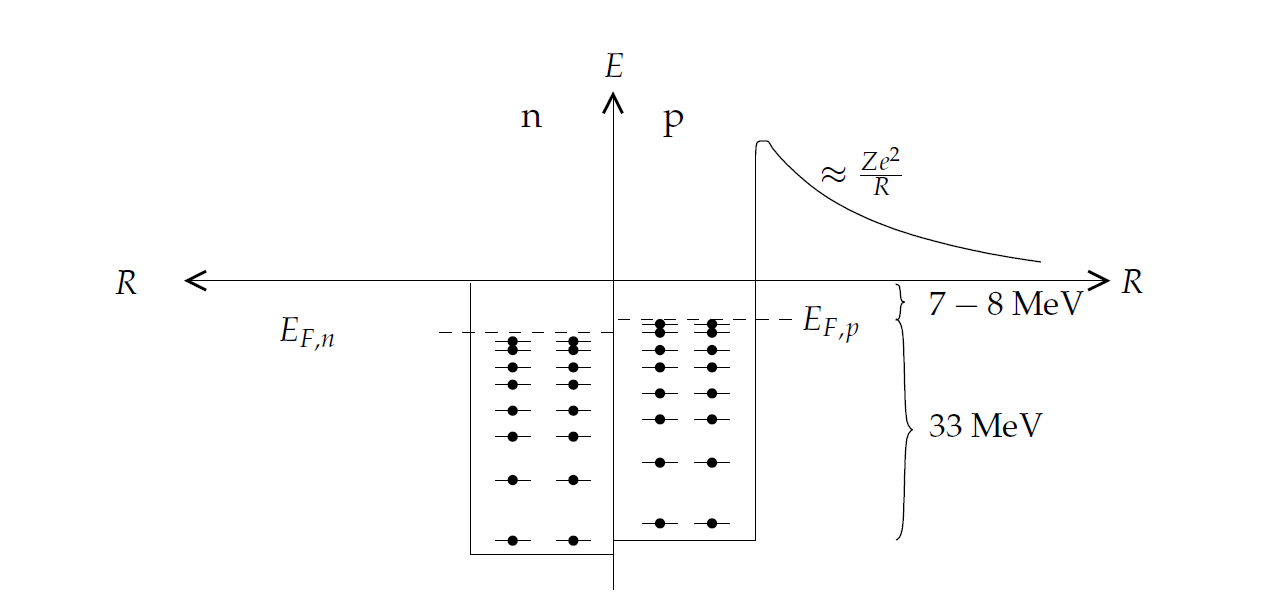
\includegraphics[width=1.0\textwidth]{img/fermigas}
	\caption{Graphische Darstellung der beiden Potentialtöpfe für Neutronen und Protonen im Fermigasmodell. \cite{fermi}}
	\label{fermigas}
\end{figure}

\subsubsection{Alpha-Zerfall}

Als erstes wird der Alpha$\left( \alpha\right) $-Zerfall erläutert. Er wurde erstmals von Ernest Rutherford beobachtet und stellt die Emission eines Heliumkerns dar. Wie in Abbildung \ref{zerfall} zu sehen tritt er nur bei relativ schweren Kernen auf. Dies kann man durch die hohe Bindungsenergie von ca. 7\,MeV des Heliumkerns begründen (siehe Abbildung \ref{be}). Mit steigender Massenzahl $A$ nimmt die Bindungsenergie ab, weshalb sich für schwere Kerne im Inneren zwei Protonen und zwei Neutronen als ein Heliumkern \glqq abkapseln\grqq\ können. Dieser Heliumkern ist jedoch nicht frei, sondern im Kernpotential gebunden. 

\noindent Stellt man sich das Potential wie in Abbildung \ref{fermigas} nach dem Fermigasmodell vor, so befindet sich das $\alpha$-Teilchen noch im Rechteckpotential des Kerns, jedoch oberhalb der 0\,MeV-Linie. Daher lässt sich quantenmechanisch eine Wahrscheinlichkeit ungleich null berechnen, mit der das $\alpha$-Teilchen auf die rechte Seite des Coulombpotentials durchtunnelt. Diese Wahrscheinlichkeit bestimmt die Zerfallsdauer. Das Grundprinzip des Alpha-Zerfalls wird also mit dem Fermigasmodell verständlich. Als allgemeine Zerfallsgleichung lässt er sich schreiben als:
\begin{align*}
^A_ZX_N\longrightarrow \,^{A-4}_{Z-2}Y_{N-2} \,+ \,^4_2\textnormal{He}_2
\end{align*}


\subsubsection{Wechselwirkung von Strahlung mit Materie}

Untersucht man die Wechselwirkung von Strahlung mit einem Target, so sind Fallunterscheidung zu machen. Die Wechselwirkung von Neutronen und leichter geladener Teilchen wie Elektronen und Positronen mit Materie ist für diesen Versuch nicht relevant. Entscheidend ist hingegen die Wechselwirkung von schweren geladenen Teilchen, hier Alpha-Teilchen und die  Kernbruchstücke des $^{252}$Cf, mit den verschiedenen Detektormaterialien. 

Schwere geladene Teilchen verlieren beim Durchqueren eines Festkörpers die meiste Energie durch inelastische Kollisionen mit den Elektronen des Festkörpers. Bei den sehr schweren Kernbruchstücken ist zudem die Wechselwirkung mit den Kernen des Mediums nicht zu vernachlässigen. Die Kollisionen mit den Elektronen können zudem in weiche und harte unterteilt werden. Bei weichen Kollisionen kommt es nur zur einer Anregung, bei harten gar zu einer Ionisation. 

Der Energieverlust schwerer geladener Teilchen kann durch die Bethe-Bloch-Formel beschrieben werden. Charakteristisch für diese ist der steile Abfall wie $1/\beta^2$ bei kleinen Energien. Bei $\beta\gamma\approx3$ wird ein Minimum erreicht, bevor der Energieverlust wieder logarithmisch ansteigt. Für sehr hohe Energien stellt sich ein Sättigungsverhalten ein.

Aus dieser Abhängigkeit des Energieverlustes folgt die sogenannte Bragg-Kurve. Diese stellt den Energieverlust pro zurückgelegtem Weg dar. Wie in Abbildung \ref{bragg} am Beispiel von Alpha-Teilchen in Luft zu sehen, ist der Energieverlust zunächst gering, da die Teilchen noch relativ viel Energie besitzen. Mit abnehmender Energie steigt der Energieverlust weiter an und die Teilchen verlieren die meiste Energie ganz zum Schluss am Bragg-Peak.

\vspace{0,3cm}

\begin{figure}[h]
	\centering
	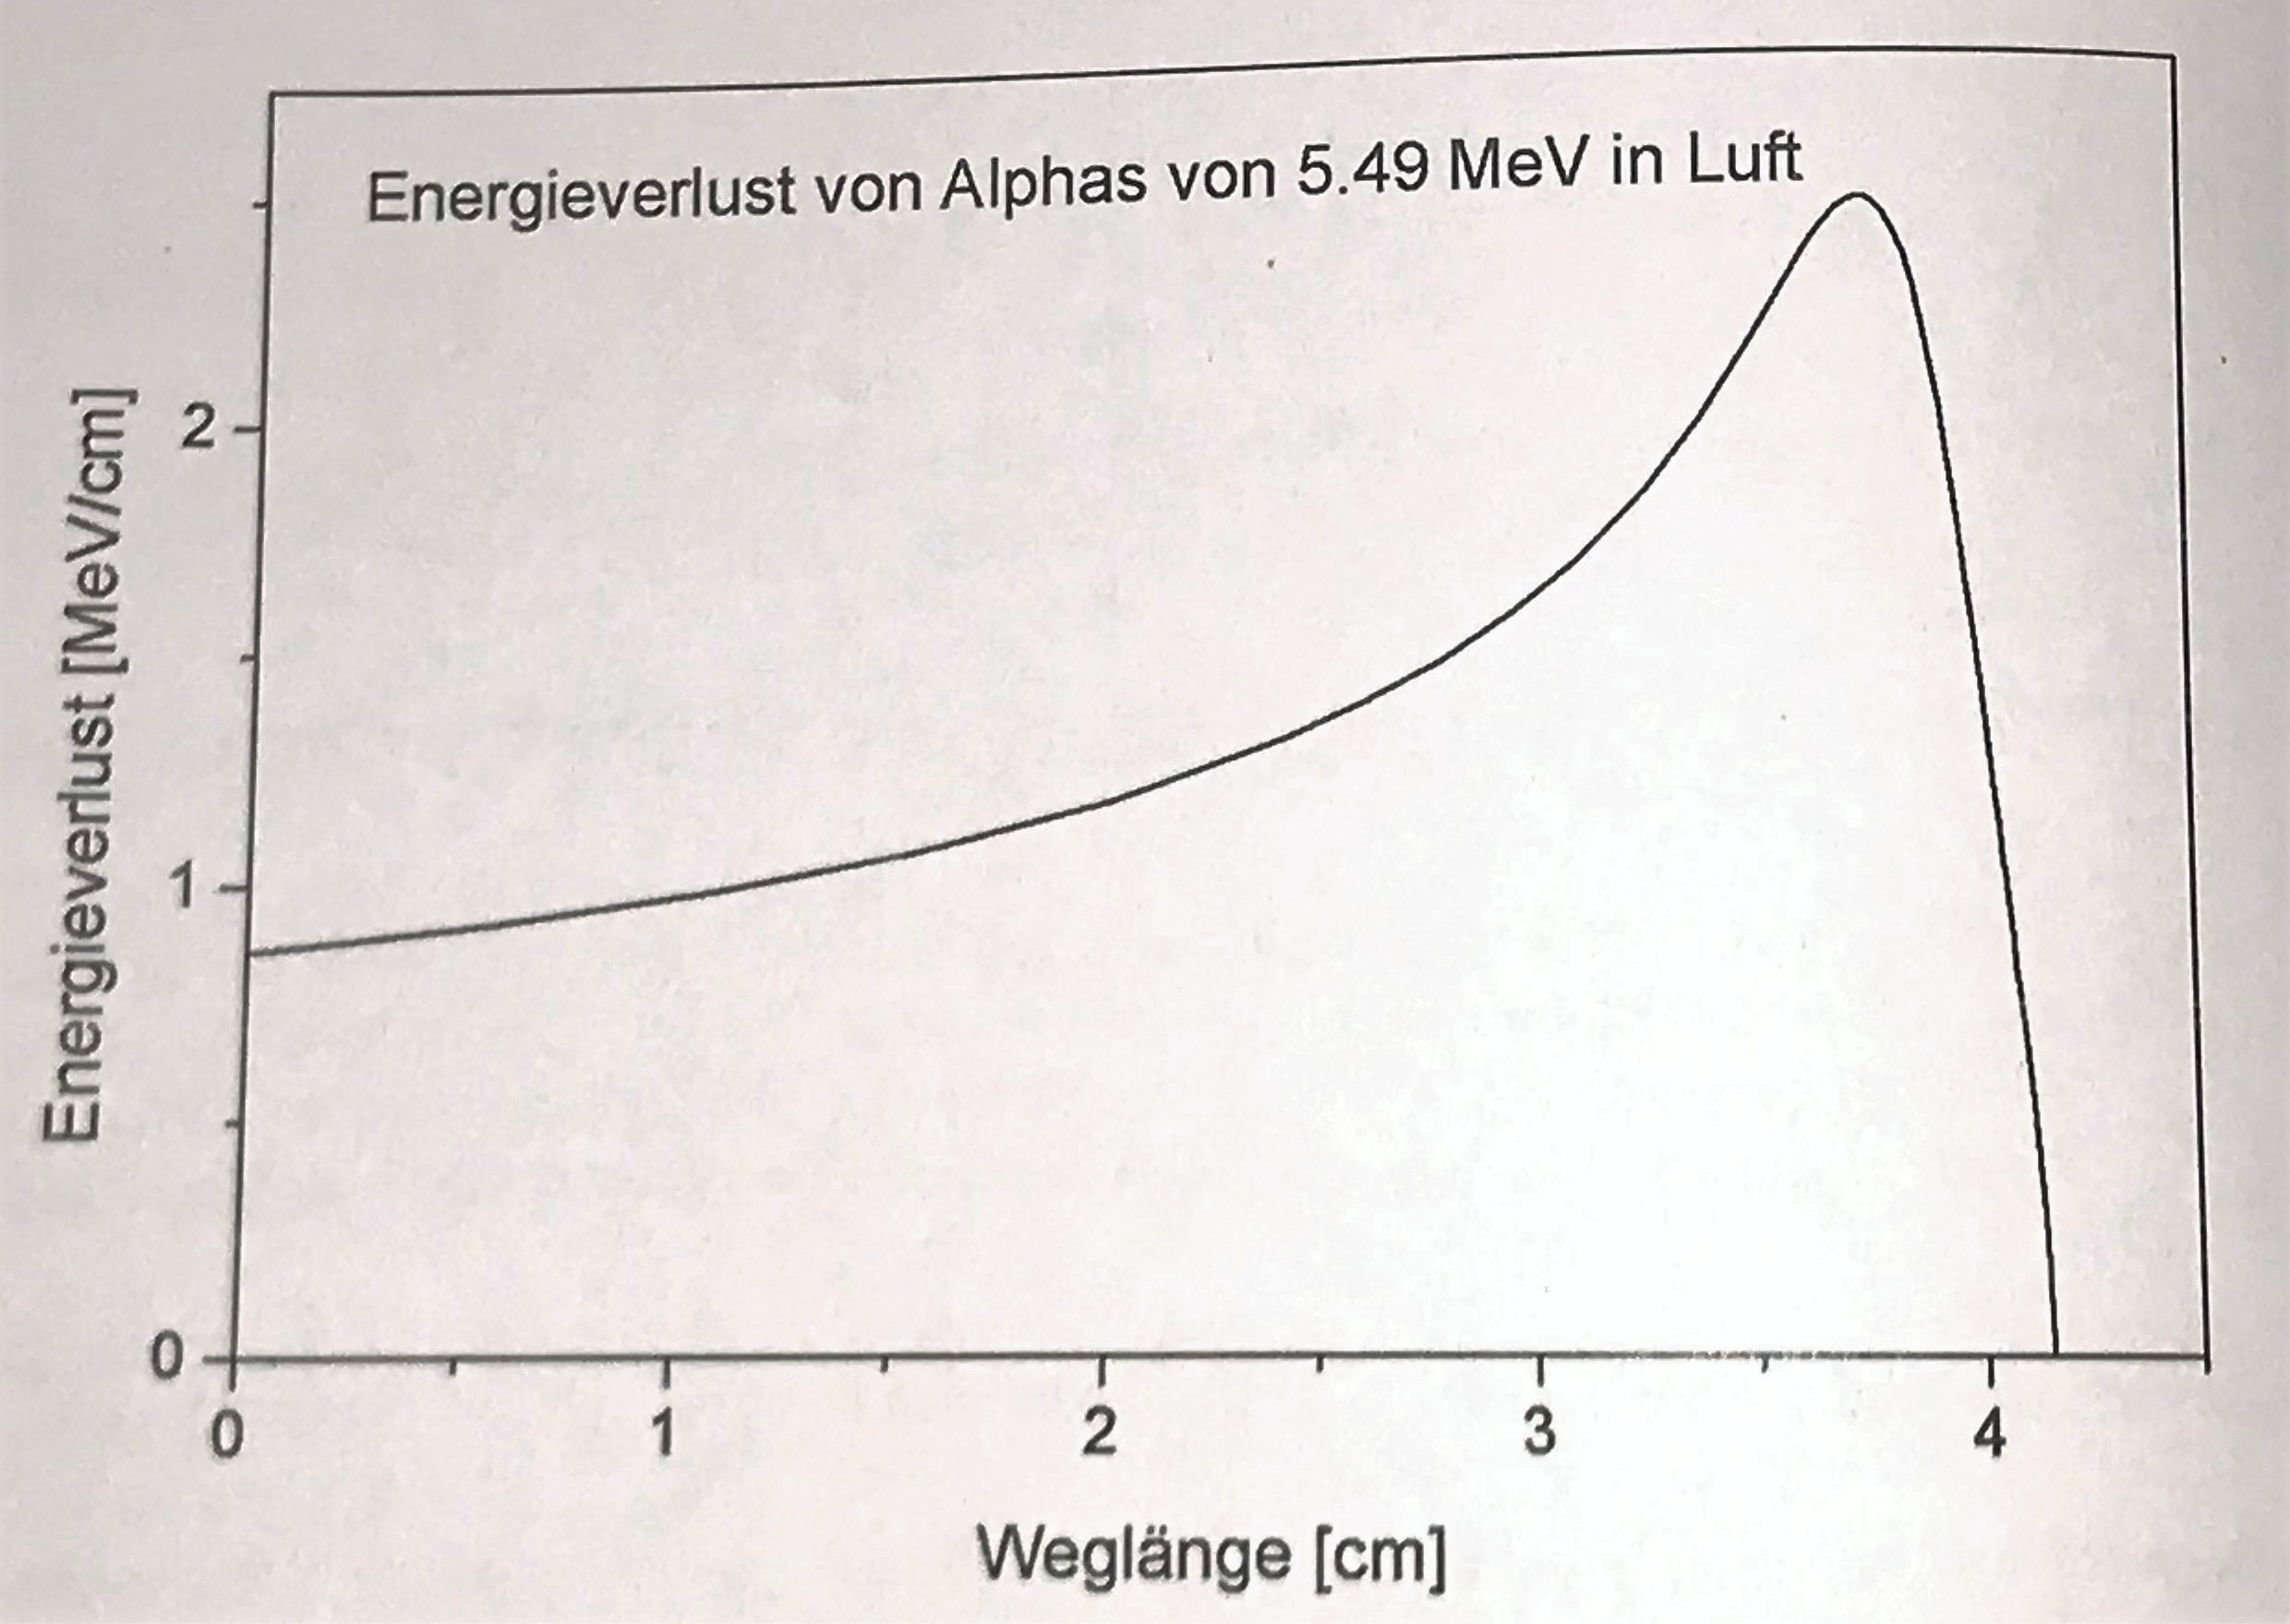
\includegraphics[width=0.8\textwidth]{img/bragg}
	\caption{Bragg-Peak von Alpha-Teilchen in Luft. \cite{bragg}}
	\label{bragg}
\end{figure}

\subsubsection{Halbleiter-Detektoren}

Ein Halbleiter-Detektor funktioniert ähnlich zu einer Gas-Ionisationskam-mer. Im Gegensatz dazu werden jedoch nicht die Ionisationen eines Gases gemessen, sondern die erzeugten Elektron-Loch-Paare in der Sperrschicht einer Halbleiter-Diode. Die zum Hervorrufen einer Reaktion notwendige Energie ist bei einem Halbleiter-Detektor um eine Größenordnung kleiner, was zu mehr freien Ladungen und einer kleineren statistischen Schwankung führt.